\begin{figure}[h]
    \centering
    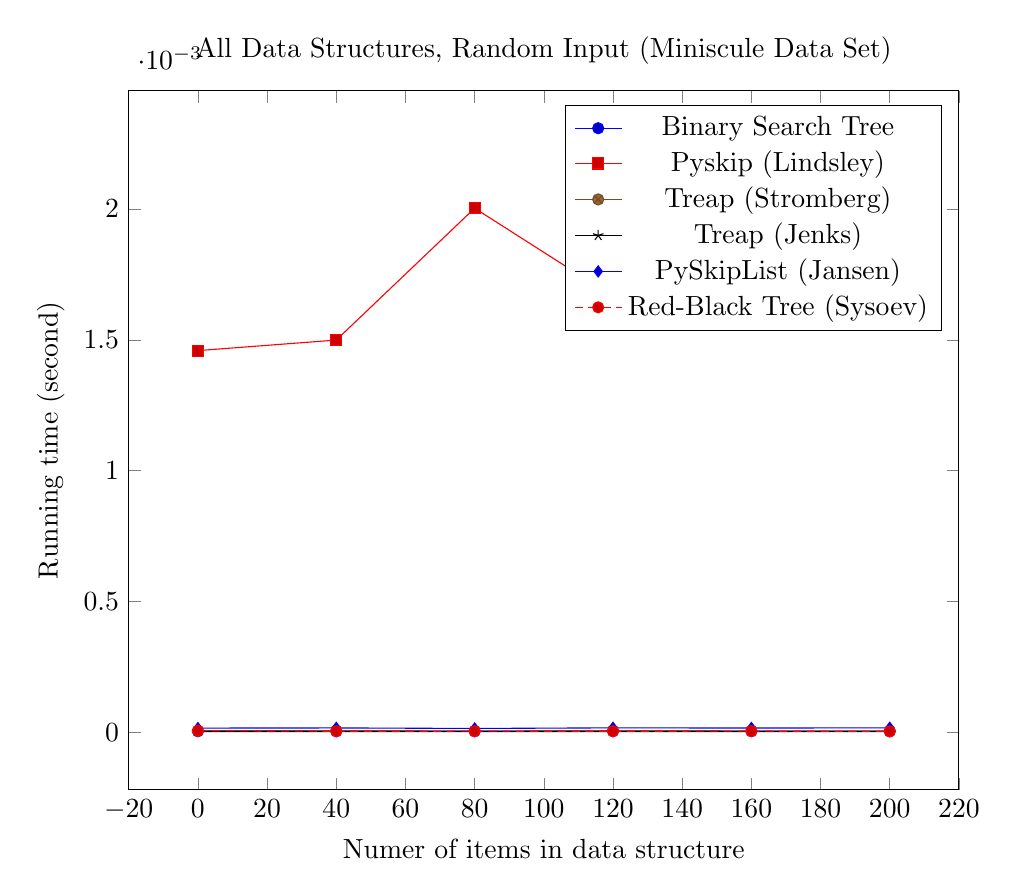
\begin{tikzpicture}
        \begin{axis}[
            xlabel={Numer of items in data structure},
            ylabel={Running time (second)},
            title={All Data Structures, Random Input (Miniscule Data Set)},
            width=\textwidth
        ]
		\addplot coordinates {
			(0, 3.553868973668606e-06)
			(40, 3.614104041022026e-06)
			(80, 3.73457417572054e-06)
			(120, 3.9152793777696985e-06)
			(160, 3.975514445120343e-06)
			(200, 3.7948092430711845e-06)
		};
		\addplot coordinates {
			(0, 0.0014585921558883553)
			(40, 0.0014989195334794037)
			(80, 0.002002996694600678)
			(120, 0.001665589964837777)
			(160, 0.0022285167867603316)
			(200, 0.002011550074164431)
		};
		\addplot coordinates {
			(0, 5.360920994179619e-06)
			(40, 6.0536242687092566e-06)
			(80, 4.939275522730658e-06)
			(120, 6.113859336054351e-06)
			(160, 5.150098258455138e-06)
			(200, 4.547747584948692e-06)
		};
		\addplot coordinates {
			(0, 2.7708130981074496e-06)
			(40, 2.409402694014684e-06)
			(80, 2.198579958290203e-06)
			(120, 2.258815025635297e-06)
			(160, 2.108227357267012e-06)
			(200, 2.1684624246121055e-06)
		};
		\addplot coordinates {
			(0, 1.572135257843499e-05)
			(40, 1.6353820785619532e-05)
			(80, 1.4275710962019517e-05)
			(120, 1.6654996122367206e-05)
			(160, 1.5962292847837567e-05)
			(200, 1.6654996122367206e-05)
		};
		\addplot coordinates {
			(0, 5.752448931961585e-06)
			(40, 3.5237514399932835e-06)
			(80, 3.915279377775249e-06)
			(120, 3.6743391083726705e-06)
			(160, 4.00563197879844e-06)
			(200, 2.9816358338430327e-06)
		};
        \legend{Binary Search Tree, Pyskip (Lindsley), Treap (Stromberg), Treap (Jenks), PySkipList (Jansen), Red-Black Tree (Sysoev)}
        \end{axis}
    \end{tikzpicture}
    \caption{Average of 10 operations, benchmarked every 40, starting at 0.}
\end{figure}